\section{Experimental methods} \label{sec:develop}
    
% Material used in the experiment

    %%%%%%%%%%%%%%%%%%%%%%%%%%%%%%%%%%%%%%%%%%%%%%%%%%%%%%%%%%%%%%%%%
    %%%%%%%%%%%%%%%%%%%%%%%%%%%%%%%%%%%%%%%%%%%%%%%%%%%%%%%%%%%%%%%%%
    %%%%%%%%%%%%%%%%%%%%%%%%%%%%%%%%%%%%%%%%%%%%%%%%%%%%%%%%%%%%%%%%%
    % SAMPLE MATERIAL

\subsection{Sample material}
    Aluminium AA2024 was machined into dimensions of \(\SI[]{100}{} \times \SI[]{100}{} \times \SI[]{5}{}\) \SI[]{}{\mm}. The surface roughness of the material was \( R_a  = \SI[]{0.754}{\micro\metre} \). The surface was not polished.  The surface residual stress baseline level measured by X-ray diffraction was  \( \SI[]{}{\sigma}  = \SI[separate-uncertainty = true]{8.15 \pm 7.80 }{\mega\pascal} \).

% Laser shock peening station setup


    %%%%%%%%%%%%%%%%%%%%%%%%%%%%%%%%%%%%%%%%%%%%%%%%%%%%%%%%%%%%%%%%%
    %%%%%%%%%%%%%%%%%%%%%%%%%%%%%%%%%%%%%%%%%%%%%%%%%%%%%%%%%%%%%%%%%
    %%%%%%%%%%%%%%%%%%%%%%%%%%%%%%%%%%%%%%%%%%%%%%%%%%%%%%%%%%%%%%%%%
    % LASER SYSTEM

\subsection{Laser system}

    A Litron LPY ST 7875-10 2HG laser was used to peen the samples. The Litron laser is a pulsed Q-switched Nd:YAG laser with an oscillator-amplifier configuration with stable resonators. The system generates pulses tens of nanoseconds in duration at \SI{532}{\nano\meter} (or \SI{1064}{\nano\meter}) with a pulse energy up to \SI{1.5}{\joule }(@\SI{532}{\nano\meter}) at \SI{10}{\hertz} repetition rate. The critical parameters of this system are summarized in Table~~\ref{tab:litronparameters}~\cite{litron}. The temporal shape of the Litron laser pulse measured by an InGaAs EOT ET-3000EXT PIN detector, and the profile of the laser pulse at \SI{36}{\milli\joule} recorded by an Allied Vision Manta G-210B ASG GigE near field camera are shown in Figure \ref{fig:profile}. The FWHM of the laser pulse is \SI{18.6}{\ns}.



\begin{table}[h!] 
\centering
        \caption[Litron~LPY~ST~7875-10~2HG parameters]{Litron~LPY~ST~7875-10~2HG parameters \protect\cite{litronmanual}}
    \begin{threeparttable}
        \begin{tabular}{|c | c|} 
        \hline
            \textbf{Parameter} & \textbf{Value} \\ [0.5ex] 
        \hline
        Repetition Rate [Hz] & 10  \\ 
        \hline
            Output Energy [mJ] & \\
            1064 nm & 3500 \tnote{a} \\
            532 nm & 1750 \\
        \hline
            Beam Diameter [mm] & 15  \\
        \hline
            Beam Divergence [mrad] & \textless 0.5 \tnote{b} \\ 
        \hline
            Pulse Width @1064 nm [ns] & 10-12 \\
        \hline
            Pointing Stability [µrad] & 25 \tnote{c} \\
        \hline
            Timing jitter [ns] & \textless 0.5 \tnote{d}  \\
        \hline
        \end{tabular}
        \begin{tablenotes}
            \small
            \item[a] Peak-to-peak Energy -- 99 \% of pulses. 
            \item[b] Full angle for 90 \% of the energy.
            \item[c] Half angle.
            \item[d] Jitter is measured concerning the external Q-switch trigger input.
        \end{tablenotes}
        
    \end{threeparttable}

\label{tab:litronparameters}
\end{table}

    %%%%%%%%%%%%%%%%%%%%%%%%%%%%%%%%%%%%%%%%%%%%%%%%%%%%%%%%%%%%%%%%%
    %%%%%%%%%%%%%%%%%%%%%%%%%%%%%%%%%%%%%%%%%%%%%%%%%%%%%%%%%%%%%%%%%
    %%%%%%%%%%%%%%%%%%%%%%%%%%%%%%%%%%%%%%%%%%%%%%%%%%%%%%%%%%%%%%%%%
    % LASER PROFILE FIGURE
        \begin{figure}[h]
        % width for 
        % you can add captions by tikzfigure
        \begin{center}

        %\begin{minipage}{.4\textwidth}
        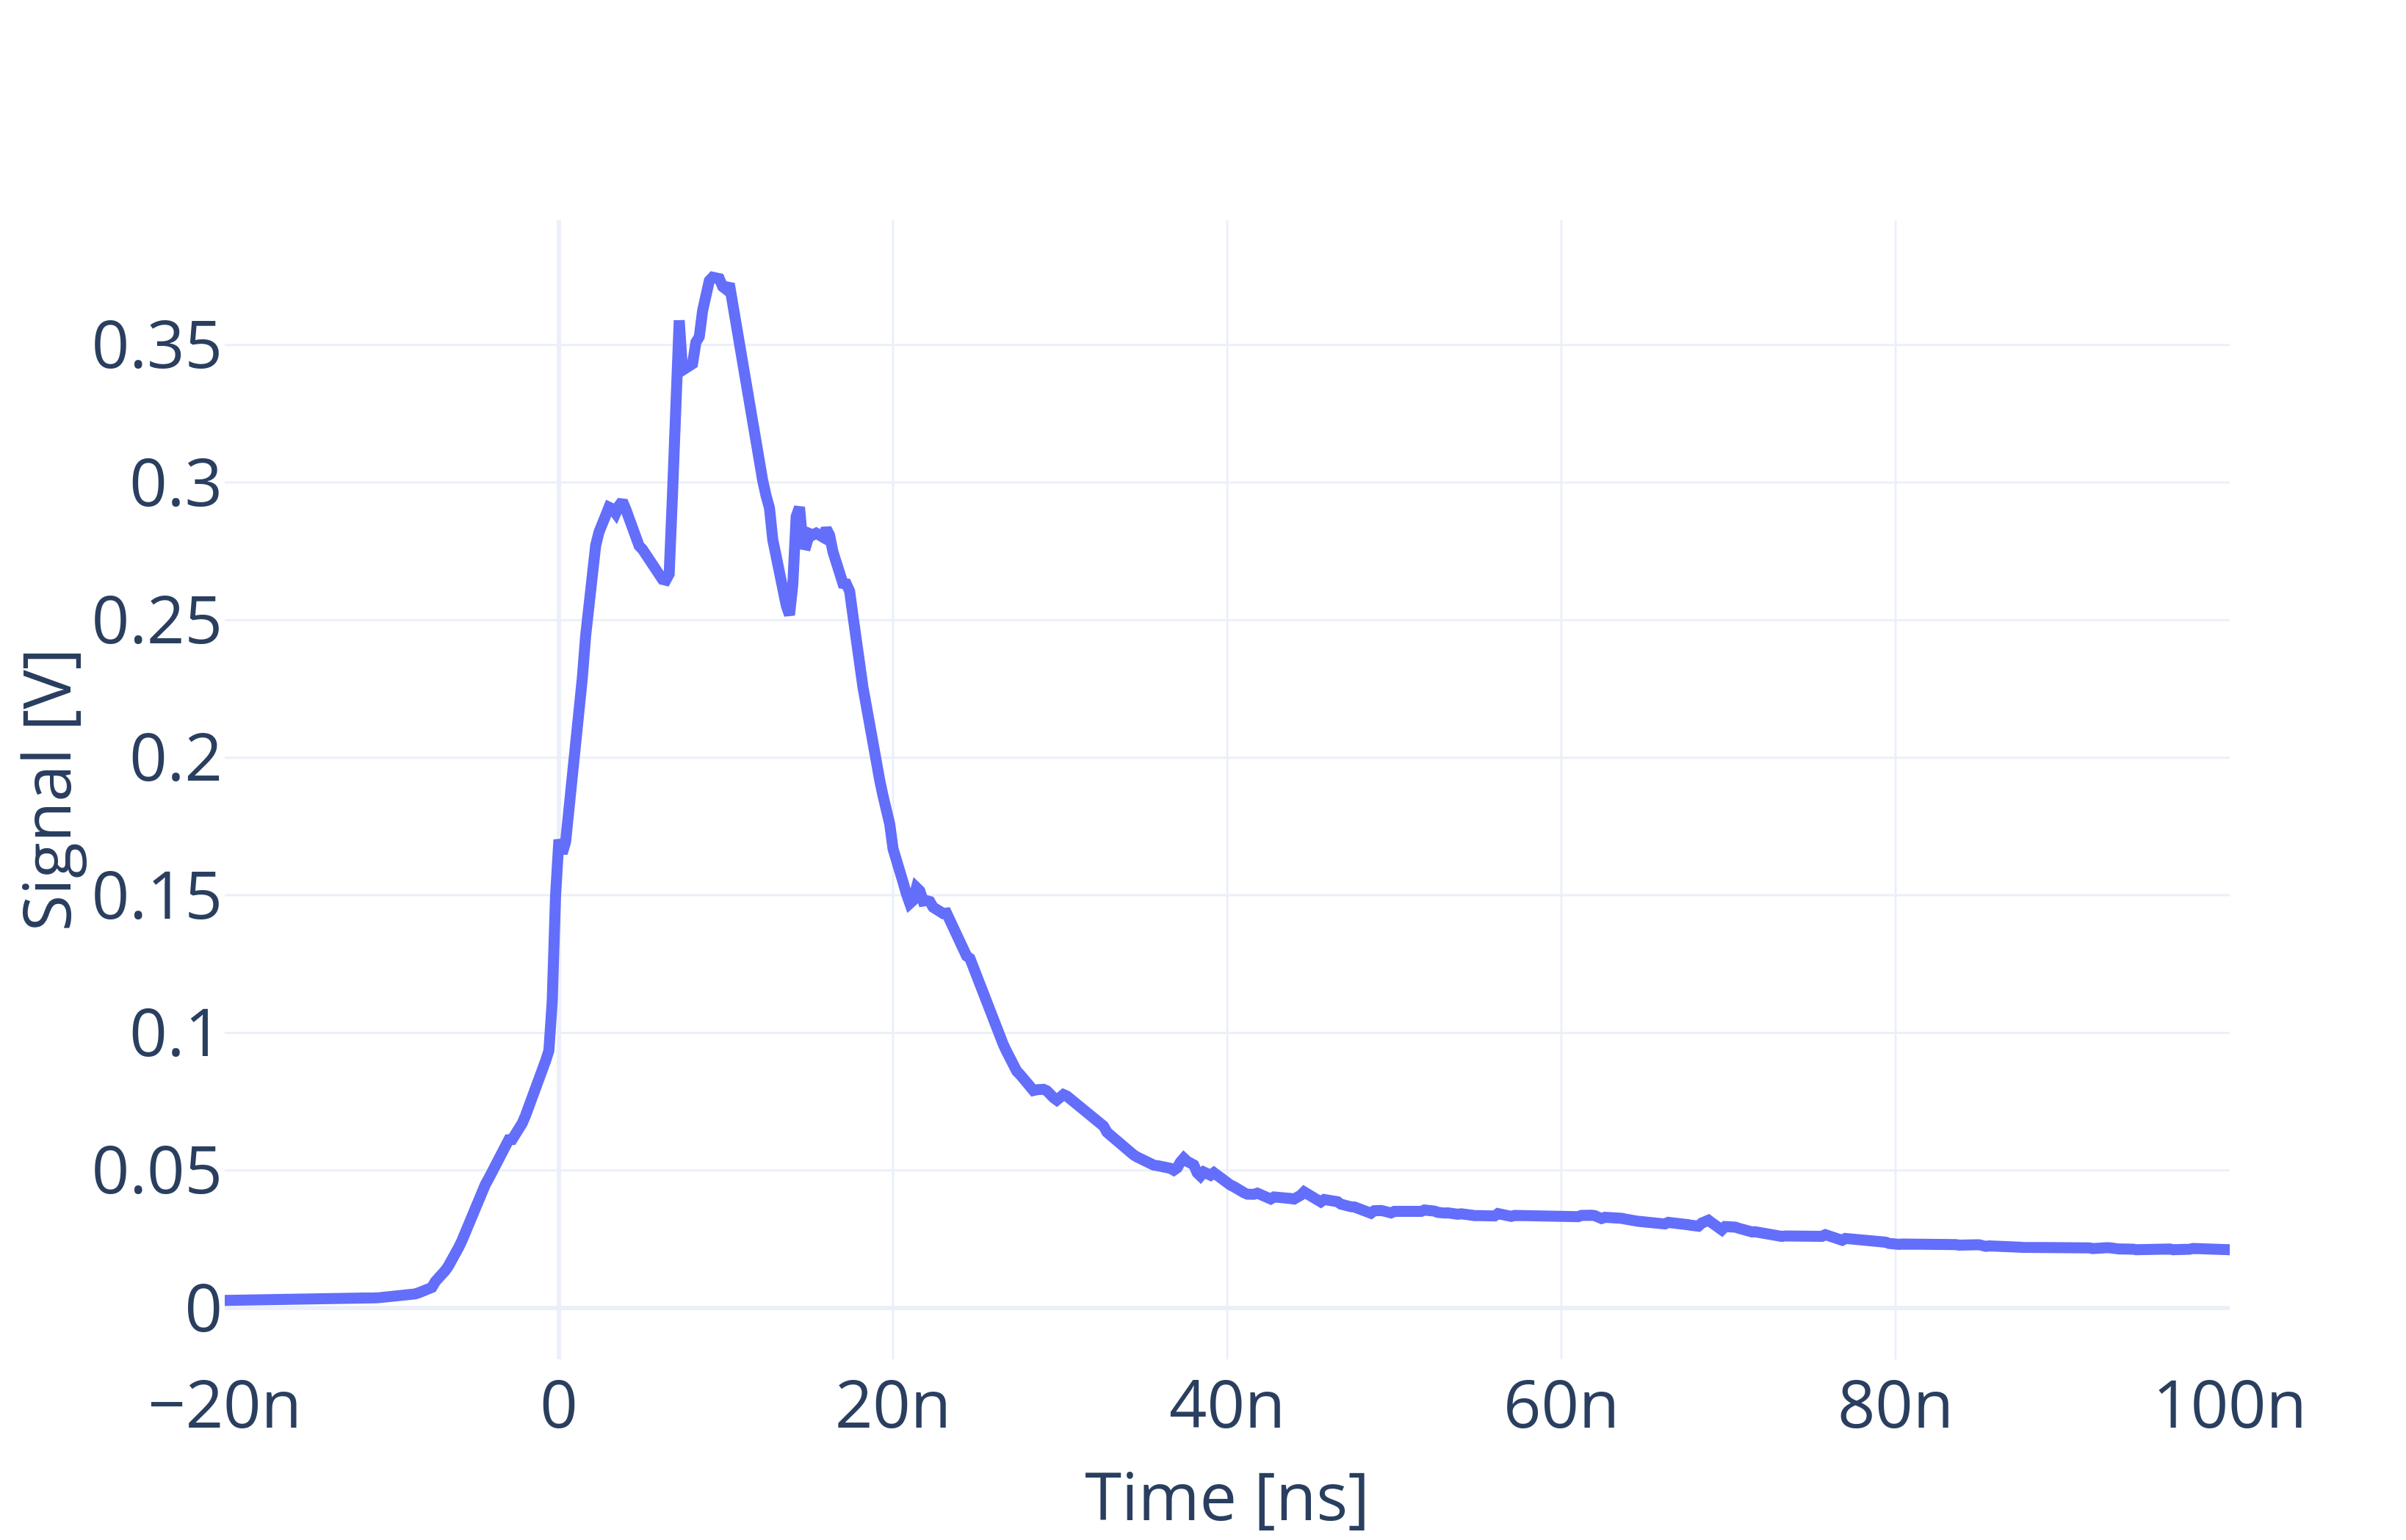
\includegraphics[width=0.27\textwidth,valign=c]{img/temporal_profile_new.png}
        \label{fig:profile}
        %\end{minipage}
        %\begin{minipage}{.4\textwidth}
        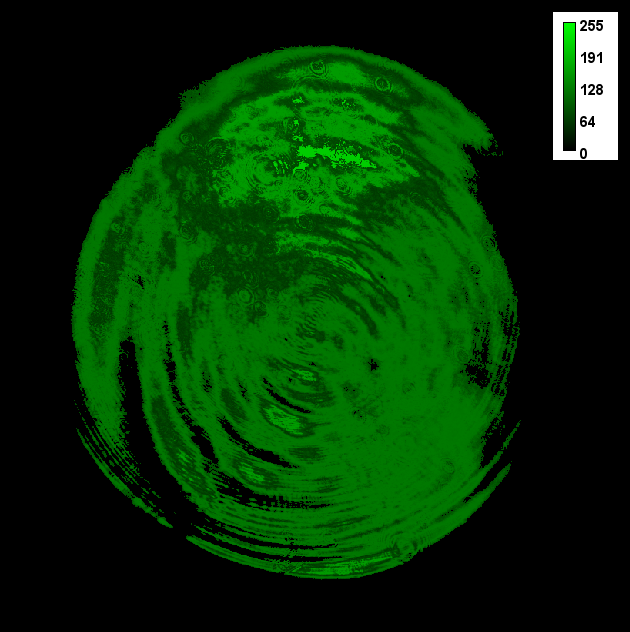
\includegraphics[width=0.15\textwidth,valign=c]{img/C2-v3_36_mJ_scale.png}
        \label{fig:profile}
        %\end{minipage}%

        \caption{Description of images from left to right: (1) Temporal shape of Litron system laser pulse (2) Near field camera profile of Litron system laser pulse}
        \label{fig:profile}
        \end{center}

        \end{figure}
    

    %%%%%%%%%%%%%%%%%%%%%%%%%%%%%%%%%%%%%%%%%%%%%%%%%%%%%%%%%%%%%%%%%
    %%%%%%%%%%%%%%%%%%%%%%%%%%%%%%%%%%%%%%%%%%%%%%%%%%%%%%%%%%%%%%%%%
    %%%%%%%%%%%%%%%%%%%%%%%%%%%%%%%%%%%%%%%%%%%%%%%%%%%%%%%%%%%%%%%%%


\subsection{Experimental setup}


\subsection{Acoustic emission}

An optical microphone is directly measuring the changes in the density of the optical medium. An optical microphone consists of a miniaturized Fabry-Pérot laser interferometer (FPI). The FPI comprises two semi-transmissive mirrors arranged at a distance matching a multiple of the laser’s half-wavelength $d$ and two lenses.

An incoming laser beam passes between the two mirrors multiple times. Part of the light in each pass is transmitted through the second surface. This process generates multiple reflected beams out of phase by a constant increment and forms interference fringes. The interference fringes form concentric circles when focused by a lens. The FPI multiple reflections follow the interference condition for thin films:

\begin{gather} \label{interference}
2d\cos\alpha = m\lambda
\end{gather} 

where:

\begin{itemize}

    \item $d$ -- distance between the two mirrors,
    \item $\alpha$ -- angle of incidence,
    \item $m$ -- order of the interference maximum,
    \item $\lambda$ -- laser wavelength.
    
\end{itemize}

Equation \ref{interference} represents the condition for the constructive interference intensity maximum \cite{fpi}.

 The optical microphone consists of two units:

\begin{itemize}
 
    \item the acoustic detection system, consisting of the optical sensor head and the driver unit comprising laser and detector,

    \item the analogue-to-digital converter with acquisition software \cite{fischer_rohringer_panzer_hecker_2017}.

\end{itemize}

 The principle of operation of the optical microphone is depicted in Figure \ref{fig:optical_microphone_principle}. The incoming sound signal causes small changes in the density of the optical medium between the two mirrors of the FPI. The FPI is inside the optical sensor head. These changes in density alter the optical index of refraction of the medium and, consequently, the laser’s propagation speed and wavelength. The distance between the two mirrors is fixed, so the change of the laser’s wavelength results in the change of the condition for the constructive interference intensity maximum, which changes the transmitted laser intensity. The laser intensity is measured with a photodiode and converted to an electrical signal.

 %% optical microphone principle 
\begin{figure}[h]
    \centering
    
\includegraphics[width=0.9\linewidth]{img/optical_microphone_principle.jpg}
    \caption{Principle of optical microphone -- the ultrasonic signal is detected optically by the change of the refractive index within a FPI etalon inside the optical sensor head \cite{fischer_rohringer_panzer_hecker_2017}}
    \label{fig:optical_microphone_principle}
\end{figure}

The Xarion Eta250 Ultra optical microphone is used. The main features of the Xarion Eta250 Ultra optical microphone are listed in Table \ref{tab:xarionparameters}~\cite{xarion_eta}. 

\begin{table}[h!] 
\centering
    \begin{threeparttable}
        \begin{tabular}{|c | c|} 
        \hline
            \textbf{Parameter} & \textbf{Value} \\ [0.5ex] 
        \hline
        Transducer type & Membrane-free, optical  \\ 
        \hline
            Frequency range &  10 Hz – 1 MHz \\
        \hline
            Dynamic range & 100 dB  \\
        \hline
            Self-noise, full bandwidth & 50 mPa  \\ 
        \hline
            Max. sound pressure for THD < 3 & 400 Pa \tnote{a} \\
        \hline
            Sensitivity & 10 mV/Pa @ 1 kHz  \\
        \hline
            Output impedance & 50 \Omega  \\
        \hline
            Polar pattern & Omnidirectional  \\
        \hline
        \end{tabular}
        \begin{tablenotes}
            \small
            \item[a] THD = Total Harmonic Distortion. 
        \end{tablenotes}
        
    \end{threeparttable}
        \caption{Xarion Eta250 Ultra optical microphone parameters \cite{xarion_eta}}
\label{tab:xarionparameters}
\end{table}